%set the master document for easy compilation
%!TEX root = ../D3_5_3.tex

The system architecture of the openETCS OBU is adopted from the system structure defined in ERA Subset-026, Chapter 2.5 \cite{subset-026}. Figure \ref{f:architecture_srs} shows which parts of the reference architecture are in the scope of the openETCS OBU model, cf.~dashed red line. Note that also specific parts of the ETCS trackside (e.g.~Eurobalise and RBC blocks) have been modeled to have an integrated test environment, cf.~dashed black line in Figure~\ref{f:architecture_srs}.

\begin{figure}[H]
\centering
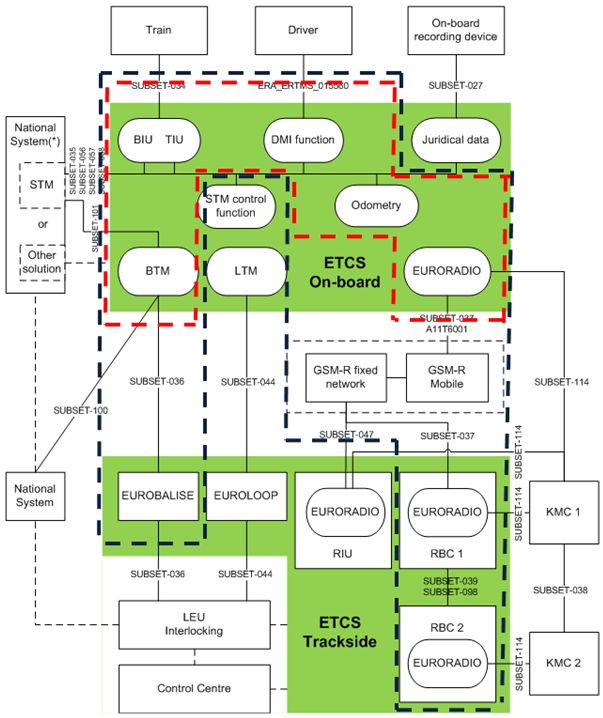
\includegraphics[width=.8\textwidth]{images/ArchitectureSRS}
\caption[Scope of openETCS OBU model system according to ERA TSI Chapter 2.5.]{Scope of openETCS OBU model system according to ERA TSI Chapter 2.5. Functional blocks in the scope of openETCS have been marked by the dashed black line. The dashed red line shows the OBU blocks in the scope of openETCS.}
\label{f:architecture_srs}
\end{figure}


\section{Top Level Architecture and External Interfaces}

Figure~\ref{f:top_level} shows the top level architecture with external interfaces E1, E2,$\ldots$, E10. The external interfaces are used for the communication between the openETCS OBU (dashed red line) and systems out of the scope of the openETCS project and the ETCS Onboard Unit System. In the following we give  brief overview of the interfaces:
\begin{figure}
\centering
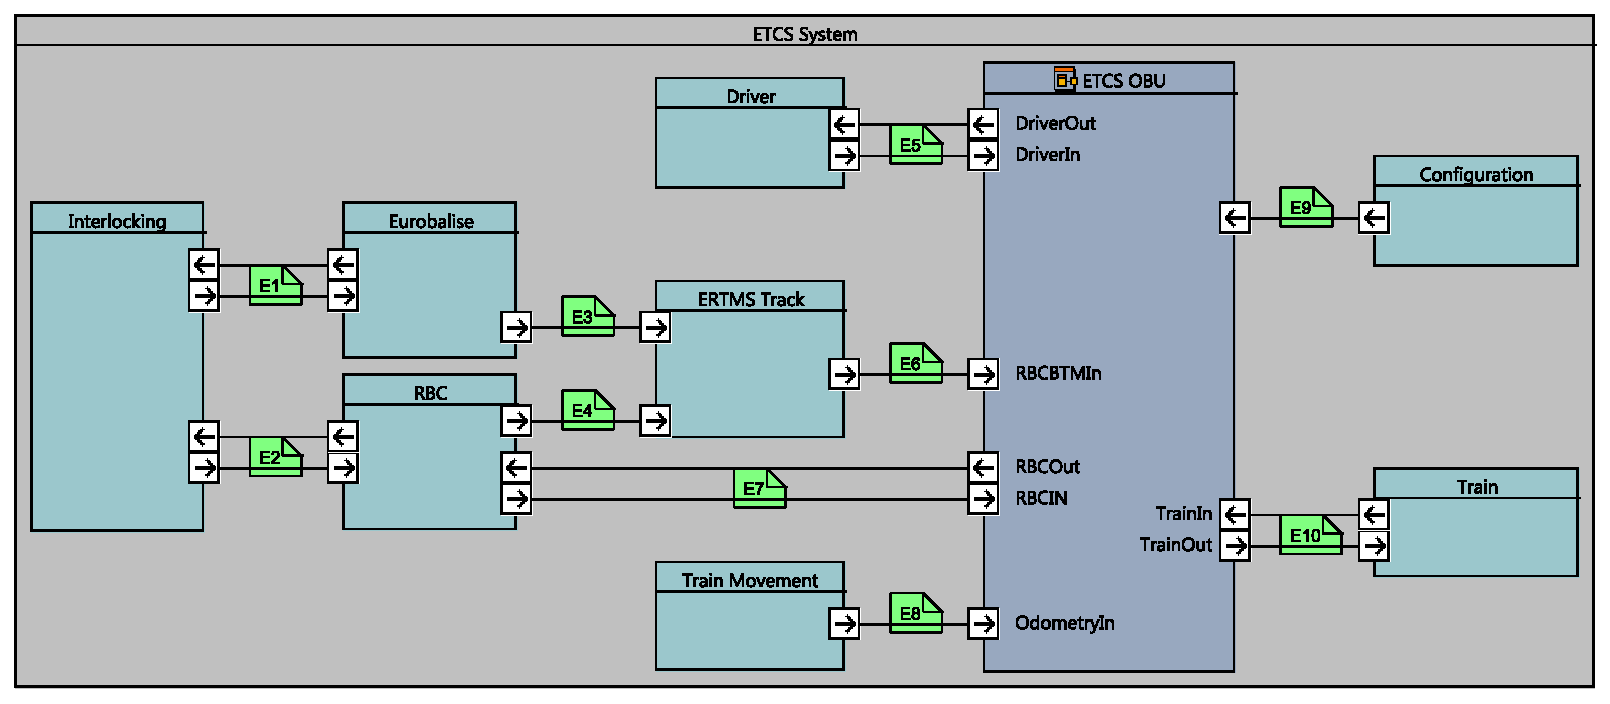
\includegraphics[width=\textwidth]{ETCS_system.pdf}
\caption{Top level architecture with external interfaces E1 to E10.}
\label{f:top_level}
\end{figure}

%\todo[inline]{Descriptions should be improved}
\begin{description}
\item[E1:] In- and out flow between the Interlocking and the Eurobalise. Only relevant for controlled Eurobalises.

\item[E2:] Input and output interface between the Interlocking and Radio Block Center (RBC).

\item[E3:] Input interface from the Eurobalise to the ERTMS Track module.

\item[E4:] Input interface from the RBC to the ERTMS Track module.

\item[E5:] This interface is used for the interaction between the driver and the display (Driver Machine Interface, DMI).

\item[E6:] This interface is a compound structure and combines the interfaces E3 and E4 to send track side messages from Eurobalises or RBC to the ETCS OBU.

\item[E7:] Input and output interface between RBC and ETCS OBU. This interface is used for the management of radio communication, e.g.~session management, and sending radio messages from the ETCS OBU to the RBC. Note that the ETCS OBU receives radio messages via interface E6.

\item[E8:] Input interface to the odometry subsystem of the ETCS OBU. Used for sending information to the train if there is any movement outside the ETCS system, e.g.~"cold movement".

\item[E9:] Input interface to the ETCS OBU to set configuration data such as fixed values, system values, national values and train configuration.

\item[E10:] Input and output interface between the ETCS OBU and the train. This interface is used for the interaction between the train and the ETCS OBU such as brake control, traction control, door control, etc.

\end{description}


\section{Functional breakdown of the ETCS OBU}

Figure \ref{f:ETCS_OBU_decomposition} depicts the functional breakdown of the ETCS OBU block shown in Figure~\ref{f:top_level}. The ETCS OBU consits out of 7 functional modules. These are:
\begin{figure}
\centering
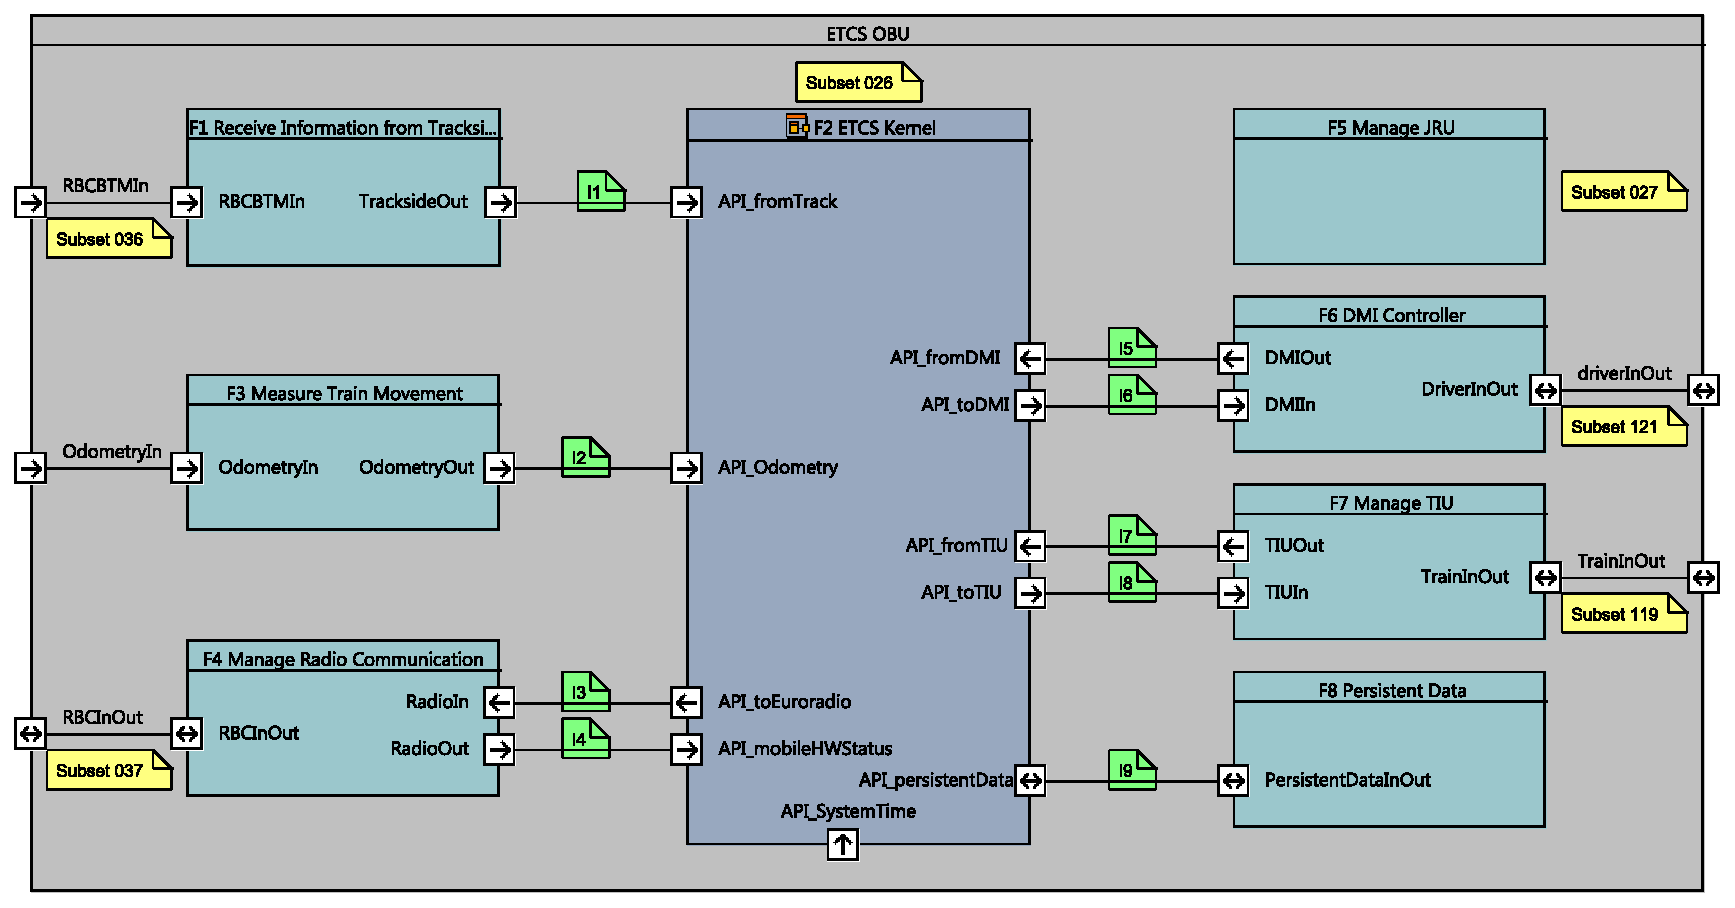
\includegraphics[width=\textwidth]{images/F2_ETCS_Kernel.pdf}
\caption{ETCS OBU system architecture view with internal interfaces I1 to I9.}
\label{f:ETCS_OBU_decomposition}
\end{figure}
%\todo[inline]{Component descriptions need to be completed}
\begin{description}
\item[F1 Receive Information from Trackside] This module is responsible for receiving RBC and BTM messages and passing these to the F2 ETCS Kernel module. A detailed description is given in Chapter~\ref{s:F1}.
\item[F2 ETCS Kernel] This module represents core component of the openETCS OBU. A detailed description is given in Chapter~\ref{s:F2}.
\item[F3 Measure Train Movement] This module provides odometry data to the F2 ETCS Kernel module.
\item[F4 Radio Communication Controller] This module controls radio transmission modules. Up to 2 modules (e.g., mobiles) can be implemented in this unit. Each module is used for setting up a communication channel between RBC and EVC. 
\item[F5 Manage JRU] This module manages the juridical date. Note that this component is not included in the functional scope of the openETCS OBU respectively project currently.
\item[F6 DMI Controller] This module implements the control of the display to the driver and the driver machine interface. 
\item[F7 TIU Controller] This module connects the train components with the EVC. It is also responsible for providing the interface to the brakes of the train.
\item[F8 Persistent Data] This module provides persistent data about the train to the ETCS Kernel.
\end{description}

These components are interacting via the internal interfaces I1 to I8. In the following we give a brief description of the interfaces.
\begin{description}
\item[I1:] Input interface that allows the F2 ETCS Kernel module to receive information from the Balise Transmission Module as well as the Radio Block Center.

\item[I2:] Input interface from the Odometry (ODO) to the F2 ETCS Kernel module.

\item[I3:] Output interface between the F4 Radio Communication controller module and the F2 ETCS Kernel module. This interface is used for radio session management and sending radio messages from the OBU to the track side.

\item[I4:] Input interface between the F4 Radio Communication Controller module and the F2 ETCS Kernel module.

\item[I5:] Input interface between the F6 DMI Controller module and the F2 ETCS Kernel module.

\item[I6:] Output interface between the F6 DMI Controller module and the F2 ETCS Kernel module.

\item[I7:] Input interface between the F7 TIU Controller module and the F2 ETCS Kernel module.

\item[I8:] Output interface between the F7 TIU Controller module and the F2 ETCS Kernel module.
\item[I9:] Input and output interface to the persistent storage of the OBU. In this storage data is made available for initialising the EVC with appropriate train status information.

\end{description}






